
\section{Rappel sur la géodynamique de l'atmosphère terrestre}%
\label{sec:structure_atmosphere}

\subsection{Composition chimique de l'atmosphère}%
\label{ssub:composition_chimique_de_latmosphere}

L'atmosphère de la terre est composée principalement de gaz. Sa composition sèche est
faite d'diazote \ce{N2} à \SI{78.087}{\percent}, de dioxygène \ce{O2} à
\SI{20.95}{\percent}, argon \ce{Ar} à \SI{0.93}{\percent}. Parmi les pourcentages restant
se trouvent le dioxide de carbone \ce{CO2} (\SI{0.041}{\percent}) et le méthane \ce{CH4},
en augmentation depuis le début de l'activité industrielle, ainsi que d'autres gaz à
l'état de trace (néon \ce{Ne}, hélium \ce{He} et krypton \ce{Kr}).  Cette composition est
dite ''sèche'' car ne prend pas en compte la vapeur d'eau, représentant en moyenne 
\SI{0.25}{\percent} de la masse totale de l'atmosphère, mais en quantité extrèmement
variable selon la localité géographique ou temporelle.

De plus, sous l'effet des radiations solaire et notamment les longeurs d'ondes
ultra-violettes (UV), de nombreux radicaux hydroxyle \ce{HO^.} sont formés et réagissent
rapidement avec les autres composants de l'atmosphère.  La quantité de dioxygène et la
présence de radicaux hydroxyle, entre autres, font de l'atmosphère un milieu à grande
capacité oxydante ayant un impact direct sur les différentes réactions pouvant avoir lieu,
aussi bien avec les gaz à effet de serre que pour les polluants organiques présents dans
les basses couches de l'atmosphère.

Enfin, il est à noter que l'atmosphère n'est pas composée que de gaz mais également de
particules solides ou liquides en suspension, que ce soit des cristaux de glace ou d'eau
liquide sous forme de nuage, mais également de ''poussières'', dont il sera question dans
cette thèse, et qui seront plus explicitement détaillées ci-après
section~\ref{sec:les_aerosols_atmospheriques}.

\subsection{Structuration de l'atmosphère}%
\label{sub:structuration_de_l_atmosphere}

\subsubsection{Une organisation stratifiée}%
\label{ssub:une_organisation_stratifiée}

À première vue l'atmosphère terrestre peut sembler homogène depuis le sol jusqu'à
l'espace. En réalité, de grande hétérogénéités sont observées à certaines altitudes,
formant des couches concentriques aux propriétés physico-chimiques très différentes, ne se
mélangeant que peu, limitant ainsi les échanges entre elles (voir
Figure~\ref{fig:chapter01/Comparison_US_standard_atmosphere_1962}).

Notamment, c'est dans la première strate atmosphérique, de \SI{0}{km} à \SI{13}{km} en
moyenne, la troposphère, que se déroulent les phénomènes météorologiques
"directement sensibles" au quotidien
(convection, formation de nuages, transport longue distance de poussières…).
C'est également la troposphère qui totalise près de \SI{75}{\percent} de la masse totale
de l'atmosphère, mais surtout en ce qui nous intéresse dans cette thèse, qui contient la
quasi-totalité de l'eau et des aérosols.

La tropopause marque la séparation entre la troposphère et la stratosphère. Elle est
notable par son changement brutal de gradient thermique (\SI{-6}{\degreeCelsius\per\km}
dans la troposphère, à \SI{0}{\degreeCelsius\per\km} dans le bas de la stratosphère).
Ceci conduit à une inversion thermique très forte, faisant de la tropopause une véritable
barrière physique. La présence de la couche d'ozone (\ce{O3}) dans la stratosphère
protège la surface de la Terre d'une partie des UV provenant du soleil, en absorbant ces
radiations. Du fait de cette absorption par l'ozone, la stratosphère se réchauffe
progressivement avec l'altitude, jusqu'à arriver à une nouvelle frontière : la
stratopause, marquée par un gradient proche de 0.

Vient ensuite la mésosphère, dénuée d'ozone et présentant donc un refroidissement car au
contact du froid de l'espace. Puis la thermosphère, qui sous l'effet des radiations
solaires, formé des ions par photodissociation, réchauffe cette zone de l'atmosphère.
C'est également à cette altitude que se produisent les aurores-boréales, lorsque les
particules du vent solaire se heurtent au champ électromagnétique terrestre à environ
\SI{100}{km} d'altitude. Puis vient l'espace extra-terrestre après \SI{600}{km}
d'altitude.

\begin{figure}[ht]
    \centering
    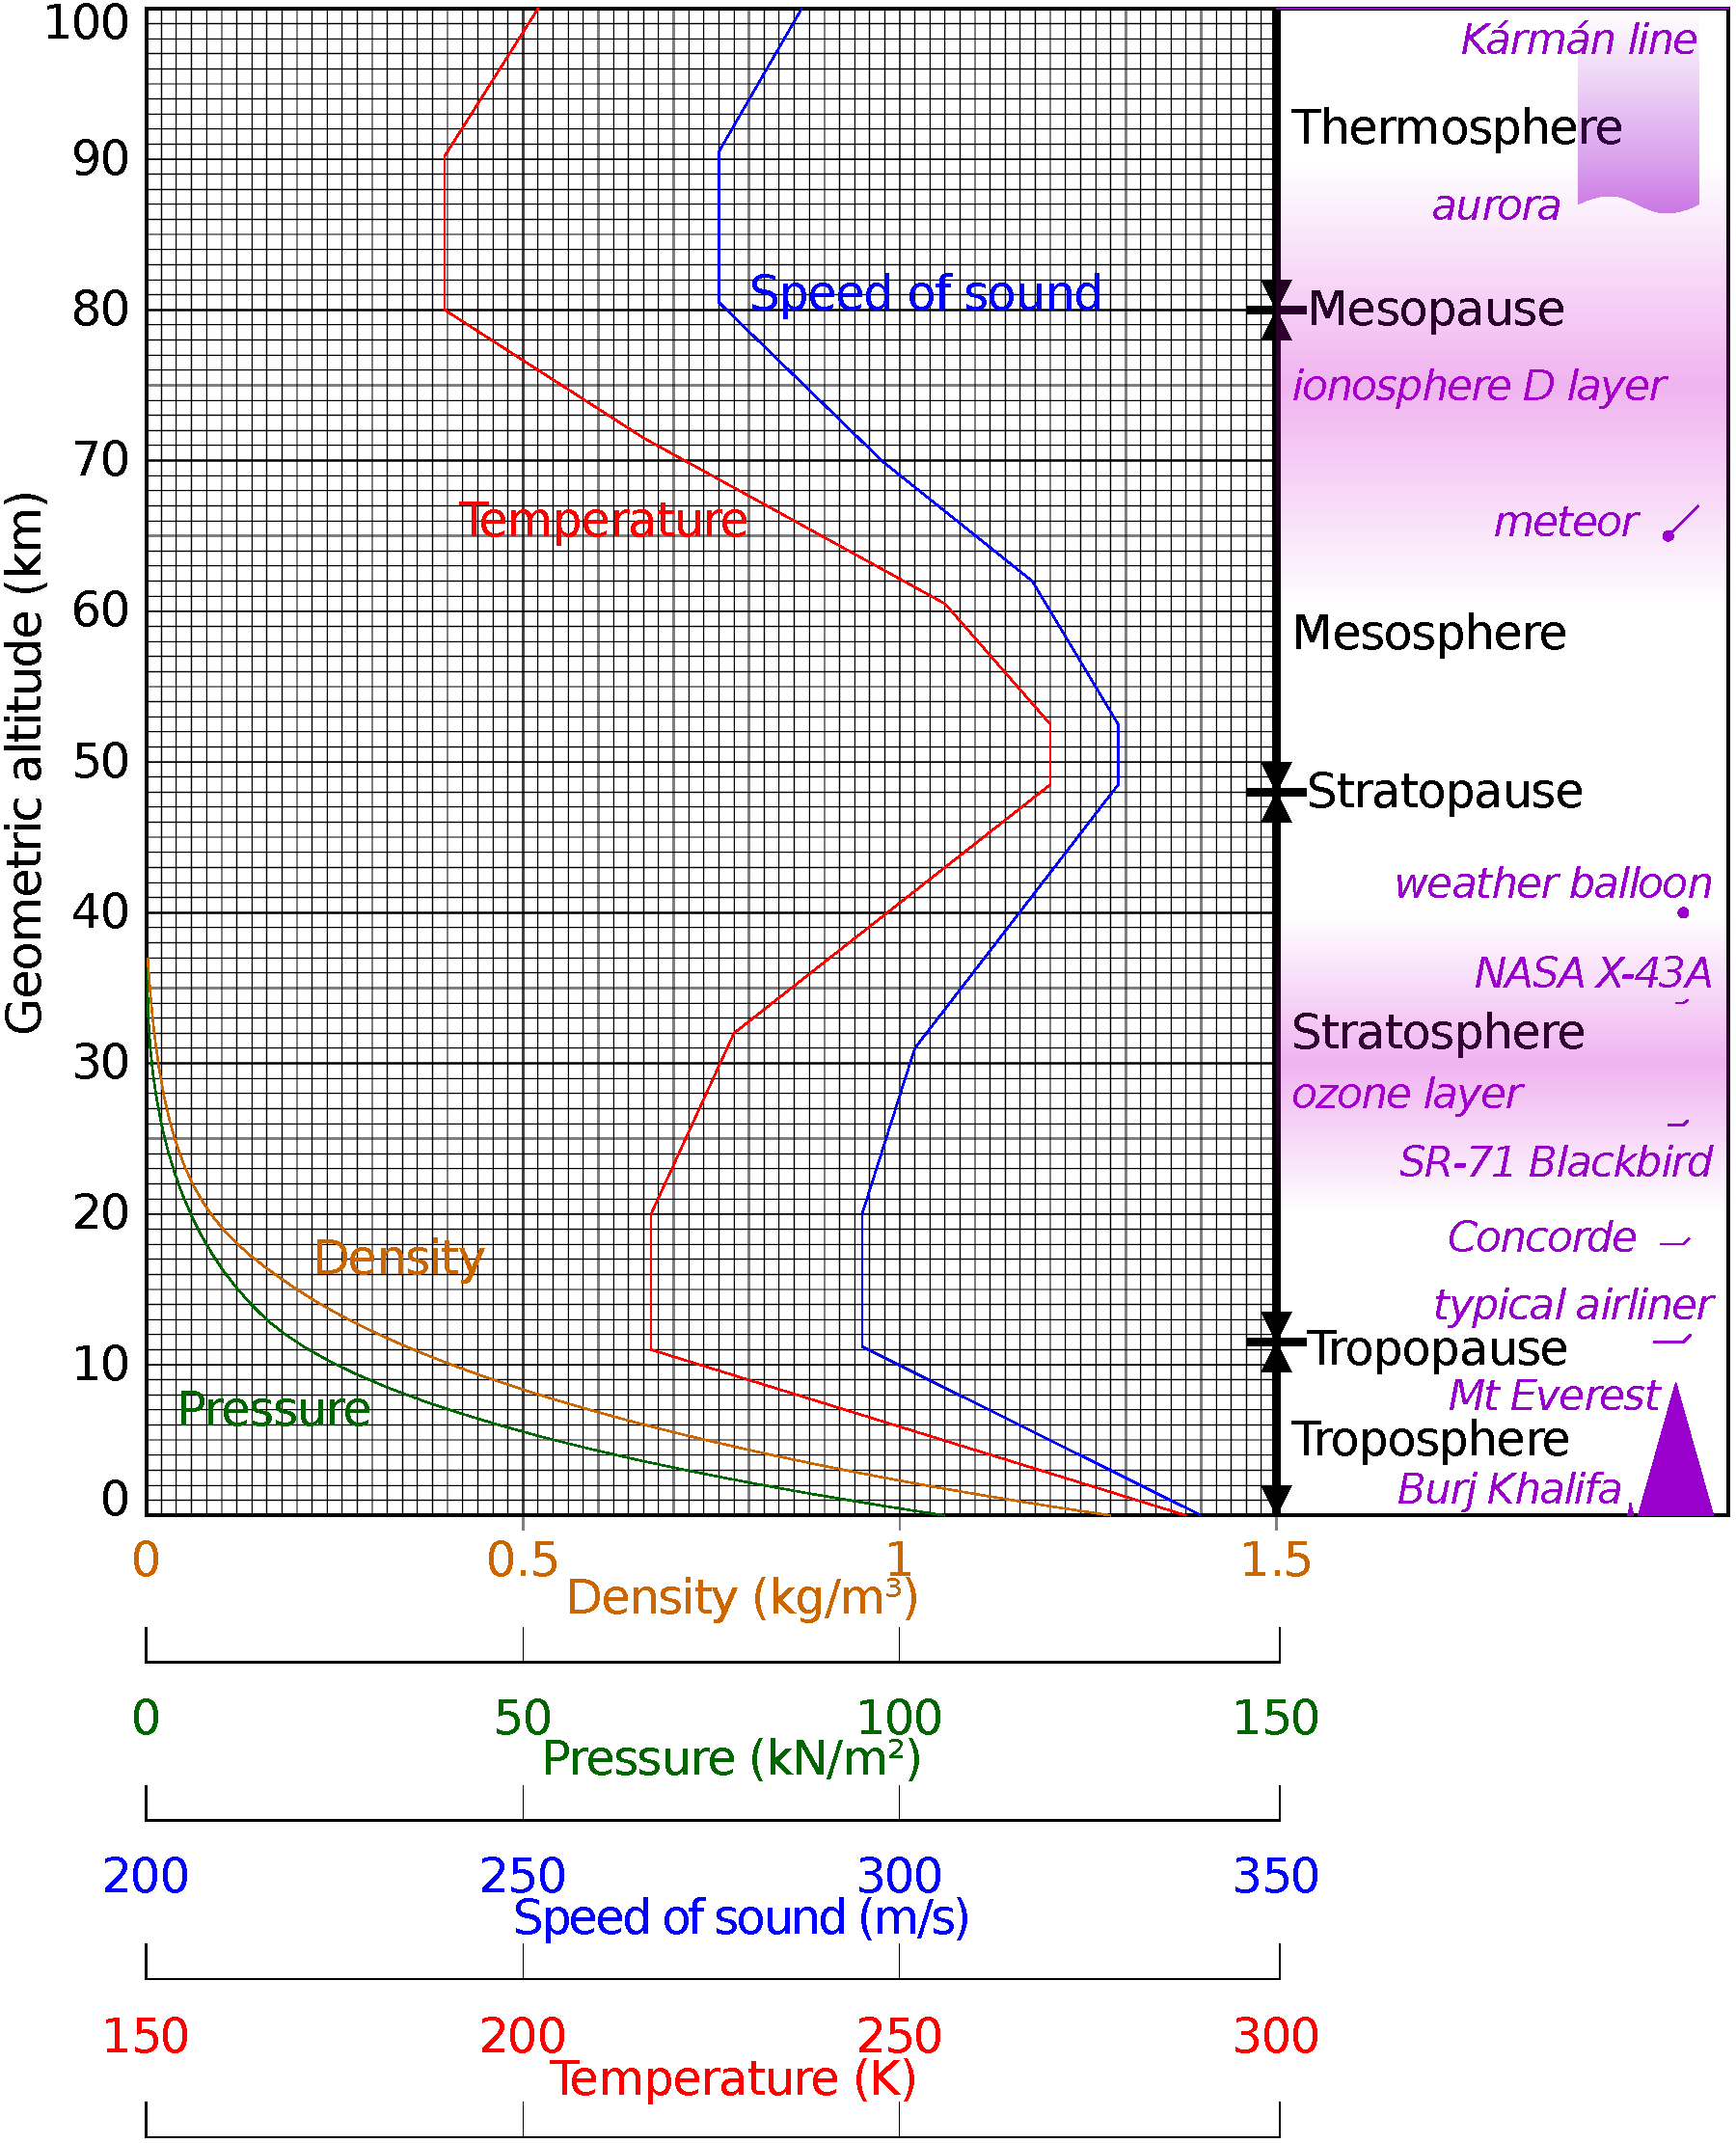
\includegraphics[width=0.6\linewidth]{chapter01/Comparison_US_standard_atmosphere_1962.pdf}
    \caption{%
        Comparaison des variables atmosphèriques selon l'atmosphère standard défini par
        l'\textit{US standard atmosphere} de 1962.
        Source:
        \href{https://commons.wikimedia.org/wiki/File:Comparison_US_standard_atmosphere_1962.svg}{wikicommons},
        par \href{https://commons.wikimedia.org/wiki/User:Cmglee}{Cmglee}, CC-BY-SA.
    }%
    \label{fig:chapter01/Comparison_US_standard_atmosphere_1962}
\end{figure}

\subsubsection{La couche limite atmosphérique}%
\label{sub:la_couche_limite_atmospherique}

À l'intérieur de cette fine couche d'environ \SI{600}{km}, seule la troposphère,
c'est-à-dire les 13 premiers kilomètres, nous est directement familière. C'est en effet
dans la troposphère que les phénomènes météorologiques auquels nous sommes habitués s'y
déroulent : nuage, vent, pluie, etc. Alors que l'atmosphère parait immense, il est
important de noter la faible hauteur de cette couche.

La partie de la troposphère directement impactée par les effets de la surface terrestre
(friction, réchauffement, turbulence) est la couche limite atmosphérique (CLA, ou
\textit{atmospheric boundary layer (ABL))}. Cette couche de quelques dizaines à centaines
de mètres, selons les lieux et période de la journée, a une dynamique rapide et
convective. En ce qui nous intéresse dans cette thèse, cela a pour conséquences que les
émissions de surface anthropiques ou naturelles, et notamment les polluants, seront
redistribués sur l'intégralité de cette hauteur.

Notamment, durant la nuit, la hauteur de la CLA est faible du fait de l'affaiblissement du
gradient thermique vertical lié à l'absence de réchauffement radiatif du sol (voir
Figure~\ref{fig:chapter01/Atmospheric_boundary_layer} et la mise en place de la couche de
surface après le couché du soleil). Après le lever du soleil, la surface se réchauffe et la
convection se met en place, rendant la CLA beaucoup plus homogène et diluant gaz et
particules dans un plus gros volume d'air. Les composés ne traversent cependant que
rarement la couche d'inversion thermique, limite entre la CLA et la troposphère libre.
Ainsi, après le couché du soleil, on observe fréquemment une couche résiduelle au milieu de
la CLA qui "capture" les composés d'une journée à une autre.

Il est à noter que des couches d'inversions thermiques à plus basse altitude peuvent se
mettre en place, notamment dans les vallées alpines. Pour un flux d'émission
constant, cela entraine donc une accumulation forte des composés chimiques dans un volume
très restreint, augmentant mécaniquement les concentrations.
\textcite{allardQualite2018} a ainsi pu montrer que le gradient thermique est l'un facteur
explicatif les plus importants pour la compréhension de la compréhension des
concentrations en vallées alpines.
%Notamment, certains jours à Passy, France, un facteur de concentration de 700 était présent entre 

\begin{figure}[h]
    \centering
    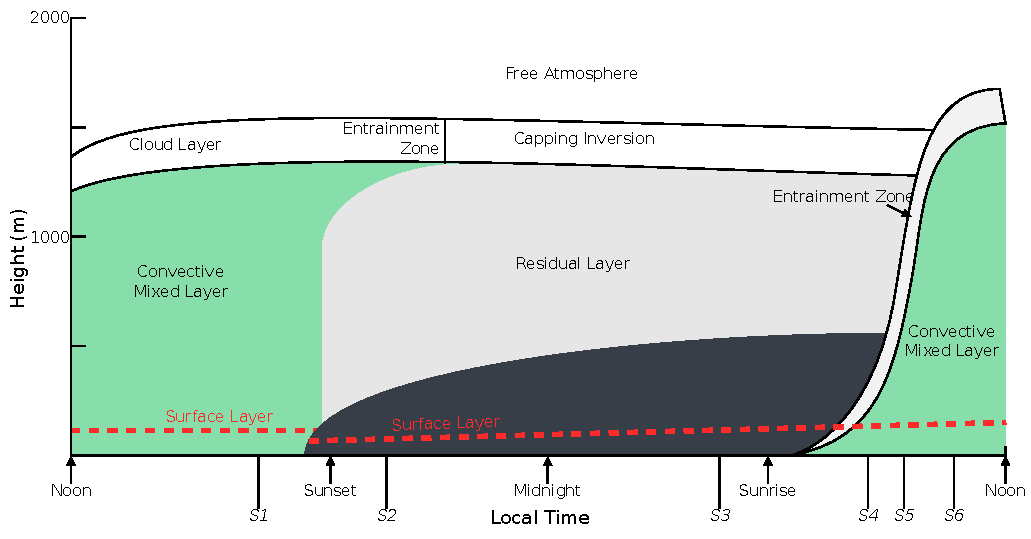
\includegraphics[width=0.8\linewidth]{chapter01/Atmospheric_boundary_layer.pdf}
    \caption{Évolution journalière schématique de la couche limite atmopshérique.
        Credit: By
        \href{https://commons.wikimedia.org/w/index.php?curid=18862904}{NikNaks} - Own
        work based on:
        \url{http://ars.sciencedirect.com/content/image/1-s2.0-S0360128504000371-gr4.jpg}.
        See also: \url{http://www.archaeocosmology.org/eng/tropospherelayers.htm}., CC
        BY-SA 3.0
    }%
    \label{fig:chapter01/Atmospheric_boundary_layer}
\end{figure}


\section{Les aérosols atmospheriques}%
\label{sec:les_aerosols_atmospheriques}
La nomenclature des aérosols est ainsi historiquement fondé sur leur taille:
\begin{itemize}
    \item \PMdix, dont le diamètre aérodynamique est inférieur ou égal à \SI{10}{\um} (petit
        grain de sable, pollens…)
    \item \PMdc, dont le diamètre aérodynamique est inférieur ou égal à \SI{2.5}{\um}
        (suie, fumée…)
    \item \PMun, parfois appellé aussi particules ultrafines (UFP), dont le diamètre
        aérodynamique est inférieur ou égal à \SI{1}{\um} (coagulation et condensation de
        vapeur…)
\end{itemize}


\subsection{Qu'est-ce qu'un aérosol?}%
\label{sub:quest-ce-quun-aerosol}

L'air que nous respirons est constitué majoritairement de gaz (\ce{N2}, \ce{O2}…) mais
également de particules solides ou liquides en suspension dans l'air. Ces particules, très
légères et de taille micrométriques ou moins, constituent une famille de composé appelé
communément particules fines, \textit{particulate matter} (PM) ou improprement particules
diesel dans le grand public.

Leurs tailles varient de quelques nanometres à plusieurs dizaines de micromètres.
À titre de comparaison, cela reviendrait à mettre dans la même catégorie une marche de
\SI{100}{m} pour aller chercher son pain à un voyage de \SI{10000}{km}.
Ainsi, cette nomenclature ''PM'' regroupe nécessairement des objets aux caractéristiques
très diverses, et comme le montre la Figure~\ref{fig:aerosolDistribution}, selon
que l'on observe les PM en s'intéressant à leur nombre, surface ou volume, l'importance
relative des classes de tailles change complètement.

\begin{figure}[ht]
    \centering
    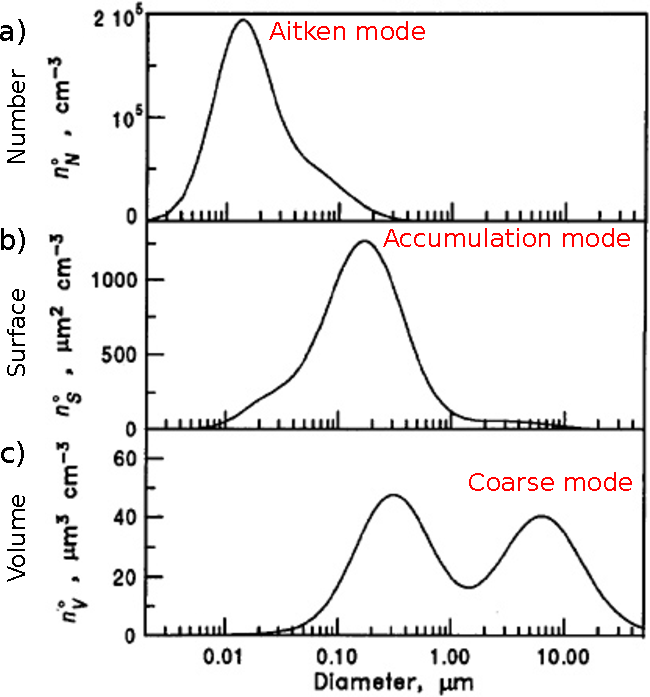
\includegraphics[width=0.5\textwidth]{aerosolDistribution.pdf}
    \caption{Distribution \textbf{(a)} en nombre, \textbf{(b)} surface, et
        \textbf{(c)} volume, pour un ensemble typique de distribution trimodale
        d'aérosols. Figure adaptée du livre de~\textcite{seinfieldAtmospheric1998}.}
    \label{fig:aerosolDistribution}
\end{figure}

Ces différents modes reflètent différents procédés conduisant à leur présence dans l'air,
allant de la nucléation à partir de composé gazeux ou de source de combustion pour le mode
dit d'Aikten, le plus fin (prépondérant en nombre), permettant par coagulation d'atteindre
des particules plus grosses (mode d'accumulation), pour enfin, lorsque la vitesse de
coagulation est suffisante, atteindre le mode grossier, pouvant également être alimenté
par diverses autres sources comme la remise en suspension de poussière ou sable par le
vent, les pollens, les activités humaines, etc, comme nous le verons plus loin.

La nomenclature des aérosols est ainsi historiquement fondé sur leur taille:
\begin{itemize}
    \item \PMdix, dont le diamètre aérodynamique est inférieur ou égal à \SI{10}{\um} (petit
        grain de sable, pollens…)
    \item \PMdc, dont le diamètre aérodynamique est inférieur ou égal à \SI{2.5}{\um}
        (suie, fumée…)
    \item \PMun, parfois appellé aussi particules ultrafines (UFP), dont le diamètre
        aérodynamique est inférieur ou égal à \SI{1}{\um} (coagulation et condensation de
        vapeur…)
\end{itemize}


Ces catégories très diverses présentent ainsi des formes variées, comme illustré par les
clichés de microscopies électroniques présentés Figure~\ref{fig:micrography}. On retrouve
des particules sphériques de petites tailles, des formes plus géométriques issues de
processus de cristallisation comme le sel marin, etc.

\begin{figure}[ht]
    \centering
    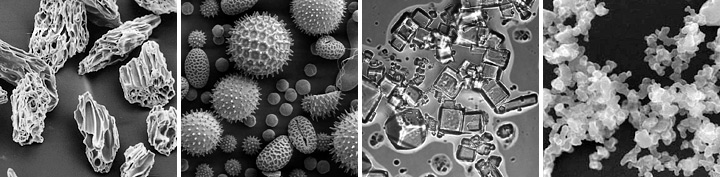
\includegraphics[width=1.0\textwidth]{aerosol_micrographs.jpg}
    \caption{Image au microscope électronique à balayage, à des échelles différentes,
        illustrant la diversité de forme des aérosols.
        De gauche à droite : cendre volcanique, pollen, sel de mer et suie. Micrographies de
        l'USGS, UMBC (Chere Petty) et de l'Arizona State University (Peter Buseck). 
        Crédit : NASA earthobservatory \url{https://earthobservatory.nasa.gov/Features/Aerosols/}.
    }
    \label{fig:micrography}
\end{figure}

\subsection{Composition chimique}%
\label{ssub:composition_chimique}

En termes d'éléments constitutifs de ces PM, il est d'usage de regrouper les espèces en
différentes classes représentant les espèces majeures de la masse des PM. La
Figure~\ref{fig:chapter01/composition_chimique} présentes les gammes de concentrations
observée à travers le monde pour différentes typologies de site de prélèvement.
On y trouve différents ions issus de la condensation de la phase gazeuse (nitrate \NOt, formé à
partir des \ce{NO_x} et l'ammonium \ce{NH_4^+}, formé à partir de \ce{NH3}) et du sulfate
\SOq, formé par condensation du \ce{SO2} mais également émis par les volcans et les
activités anthropiques).
Une part également importante de la masse provient de la matière carbonée, notée ici
carbone organique (ou \textit{organic carbon} OC). Ce terme regroupe un nombre extrèmement
important d'espèce chimique comportant une chaine carbonée, de l'oxygène et
de l'azote. On y retrouve par exemple la cellulose ou autres sucres issues de sa
dégradation par combustion (lévoglucosan, mannosan, galactosan), des "polyols" (arabitol,
mannitol, etc) émis par les bactéries ou champignons~\autocite{samakePolyols2019}, ou encore
d'autres famille de molécule comme les alcanes, hopanes, composé aromatique polycyclique
ou même pesticide. Cette matière carbonée est souvent exprimée en terme de matière
organique (MO, ou \textit{organic matter} OM) prenant en compte la masse du carbone mais
également des autres atomes (oxygène, azote…) via un facteur correctif variant entre 1.2
et 2.3 suivant les lieux de prélèvement.
Mais le carbone est également présent sous forme plus "pure" (i.e. sans oxygène ni azote).
On parle alors de carbone élémentaire (\textit{elementary carbon} EC) lorsqu'il est mesuré
par méthode thermique, et de carbone noir (\textit{black carbon} BC) lorsqu'il est mesuré
par méthode optique. Cette distinction EC ou BC provient du fait qu'il existe un continuum
entre le carbone organique et le carbone élémentaire, et que chacune des méthodes
d'observation implique un seuil de différentiation entre les deux catégories.
Finalement, d'autres ions sont également présents, comme le sodium \ce{Na^+}, le chlore
\ce{Cl-}, le magnésium \ce{Mg^2+}, etc. mais également de nombreux éléments métalliques
comme le cuivre \ce{Cu}, l'aluminium \ce{Al}, le titan \ce{Ti}, le calcium \ce{Ca}, le fer
\ce{Fe}, etc.

La composition chimique d'un aérosol dépend de ses sources d'émissions (voir
également~\ref{sub:profile_chimique_des_sources_d_émissions_courantes} mais également des
différents processus bio-physico-chimiques présents dans l'atmosphère. En effet, sous
l'effet des radiations solaires, de la capacité oxydante de l'atmosphère ou des
micro-organismes vivant dans l'air, la composition chimique des aérosols évolue au cours
de sa vie. On parle d'\textit{aérosol primaire} lorsque la chimie reflète celle des
sources d'émission, et d'\textit{aérosol secondaire} lorsque les composés chimiques
proviennent de réactions ayant eu lieu dans l'air.

Cette sensibilité aux sources d'émissions explique en partie la variabilité observée sur
la composition chimique et sa sensibilité à la typologie du site d'étude. Les sites
marins présentant davantage de sels marins, les sites proches des déserts de sable
davantage de poussière minérale, les sites urbains davantage de marqueur de combustion
(EC), etc.

\begin{figure}[htpb]
    \centering
    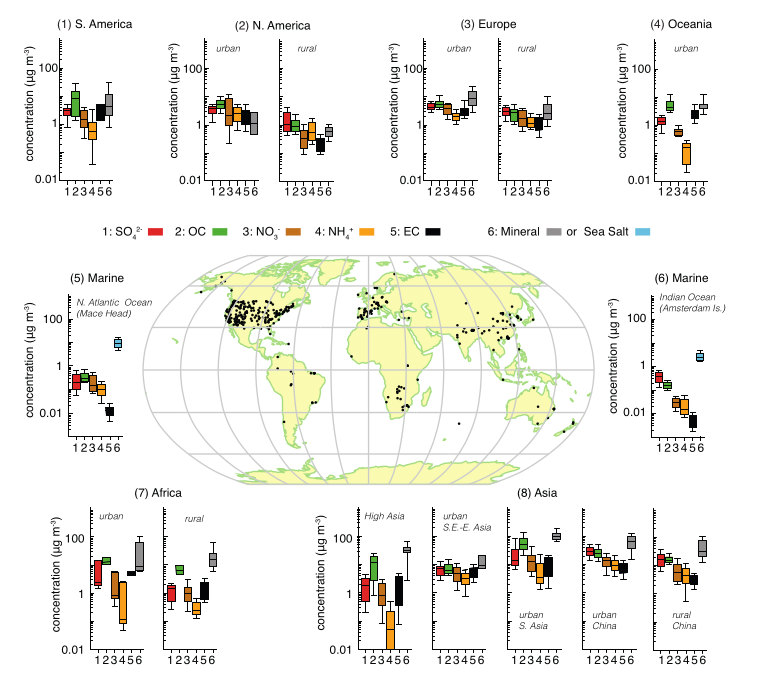
\includegraphics[width=1.0\linewidth]{chapter01/composition_chimique.png}
    \caption{Composition chimique majeurs de la masse des \PMdix{} pour différentes
        typologies de sites de prélèvement. Crédit: \cite[figure 7.13]{boucherClouds2013},
        agrégeant 113 études sur au moins une année de prélèvement, entre 1993 et 2012.}%
    \label{fig:chapter01/composition_chimique}
\end{figure}

\subsection{Impacts des aérosols sur l'écosystème terrestre}%
\label{sub:impacts_des_aérosols_sur_l_écosystème_terrestre}

\subsubsection{Impacts climatiques}%
\label{ssub:impacts_climatiques}

Les aérosols sont des éléments essentiels de la machine climatique terrestre de part leur
interaction avec le rayonnement solaire et donc leur impact sur le bilan radiatif de la
Terre, mais également par leur interaction très forte avec la dynamique des nuages, au
point que les rapports du GIEC traitent dans le même chapitre les nuages et les aérosols.

\paragraph{Impact radiatif}%
\label{par:impact_radiatif}

De part leur faible taille, les aérosols diffusent le rayonnement incident et agissent donc
comme "bouclier thermique", ré-émettant une partie du flux solaire entrant dans l'espace,
conduisant ainsi à un refroidissement de l'atmosphère.
Cependant, les aérosols absorbent aussi une partie du rayonnement incident, augmentant
l'agitation thermique et donc conduisant à un réchauffement du climat.
Ces deux effets agissent de concert, à différentes altitudes de l'atmosphère, et selon la
composition chimique des aérosols.
Enfin, la déposition des aérosols, et notamment du black carbone, sur la neige ou les
glaces des banquises induit un effet bien connu de rétroaction positive : le carbone
absorbant le rayonnement normalement réémis par les surfaces blanches diminue l'albédo de
la surface, augmente localement la température, fait fondre la glace, découvrant des
surfaces plus sombre (roche ou océan), absorbant davantage de rayonnement, conduisant à
un réchauffement accru, etc.

\paragraph{Noyaux de condensation des nuages}%
\label{par:noyaux_de_condensation_des_nuages}

Mais les aérosols, grâce à leur taille et leurs ions, permettent également de baisser
l'énergie d'activation nécessaire à l'agrégation de la vapeur d'eau sous forme liquide en
gouttelettes, puis goutte, facilitant l'apparition des nuages. Ainsi, les aérosols agissent
comme noyaux de condensation des nuages (CCN pour \textit{cloud condensation nuclei}). Or
les nuages empêchent certes les infrarouges terrestres de repartir vers l'espace, mais
présentent également un albédo élevé, renvoyant une grande partie du rayonnement à courte
longueur d'onde du soleil vers l'espace. L'effet observé est donc un refroidissement du
climat.
Aussi, pour une même quantité d'eau, le nombre de CCN disponible conditionne la taille des
gouttelettes des nuages, et donc leur taille, durée de vie et probabilité de se
transformer en nuage précipitant.

\paragraph{Impacts sur le dérèglement climatique en cours}%
\label{par:impacts_sur_le_dereglement_climatique_en_cours}

Pour ces différents aspects, très brièvement exprimé ici, l'impact total des aérosols sur
le climat est connu avec une incertitude élevée. 

Notamment, leur contribution à la différence du forçage radiatif entre 1750 et 2011 --qui
est de \SI{2.29}{\W\m\squared}-- s'estime entre
\SIrange[range-phrase=~et~]{-0.77}{0.23}{\W\per\m\squared}, avec un forçage négatif pour
les poussières minérales, le sulfate, nitrate et carbone organique, mais positif pour le
carbonne noir.  Quant à leur rôle sur la dynamique des nuages, il s'estime entre
\SIrange[range-phrase=~et~]{-1.33}{-0.06}{\W\per\m\squared}, mais présente des
incertitudes plus élevés dû fait de la complexité à prendre en compte ces phénomènes dans
les modèles de climat. C'est actuellement le forçage radiatif le moins bien connu de la
machine climatique Terrestre.

\subsubsection{Impacts environnementaux}%
\label{ssub:impacts_environnementaux}

La durée de vie des aérosols dans l'atmosphère entre leur émission et leur déposition est
de plusieurs jours. Dans ce délai, la circulation atmosphérique les déplacant sur des
distances pouvant être de plusieurs milier de kilomètre. Il n'est pas rare par exemple en
Europe d'avoir des épisodes de dépositions de sable provenant du désert saharien. Ce
déplacement longue distance d'aérosols est même un des mécanismes clef de certains "bloom"
de phytoplancton, apportant d'importante quantité de nutriment à la surface de l'océan (en
métaux et phosphate notamment).
Plus spectaculaire, les cendres volcaniques relarguées dans l'atmosphère suite à de
violentes éruptions, en plus de leur impact climatique potentiel, peuvent occasioner des
pluies acides du fait de la présence en quantité de sulfate dans ces cendres.
Autre exemple marquant, le nitrate est l'un des éléments limitant de la croissance des
plantes en prairie d'altitude. Or une partie importante de ce nitrate est apporté par
déposition de nitrate d'amonium particulaire provenant du transport longue distance.

Cette liste n'a pas pour but d'être exhaustif mais uniquement de présenter à quel point
les aérosols et leur composition chimique variée impacte directement de nombreux
écosystèmes terrestres, qu'ils proviennent de sources anthropiques comme c'est le cas pour le
nitrate, ou de sources naturelles.

\subsection{Impacts sanitaires}%
\label{sub:impacts_sanitaires}

Finalement, l'impact sanitaire des aérosols sur la population humaine a commencé à être
un sujet de recherche suite à l'industrialisation et aux épisodes de "smog" causant la
mort de plusieurs personnes à Engis (Meuse, Belgique) en 1930, Donora (Pennsilvanie, USA)
en 1948 ou encore le plus connu "Great smog of London", en 1952. Durant ces épisodes de
pollutions, il est important de noter que la sur-mortalité due à l'exposition aigue
durant l'épisode de pollution est très importante (jusqu'à 3 fois supérieure à la normale
pour le smog de Londres), mais que la surmortalité persiste dans les mois qui suivent
--pendant près d'un an pour le smog de Londres, alors même que les niveaux de pollutions
étaient revenus à leurs états pré-décembre 1952 \autocite{bellReassessment2001}.  Ces
épisodes de pollutions intenses marquent le début de la prise de conscience par la
population de la problématique de la pollution de l'air et ont conduit à la première
législation anglaise en matière de qualité de l'air en 1956 avec le \textit{Clean Air
Act}. Aussi, des programmes de mesures de la qualité de l'air pour différents polluants
ont émergés et les actions misent en œuvre au niveau national et international ont permis
en Europe une amélioration très sensible de la qualité de l'air
(Figure~\ref{fig:chapter01/tendance_polluants}).

\begin{figure}[ht]
    \centering
    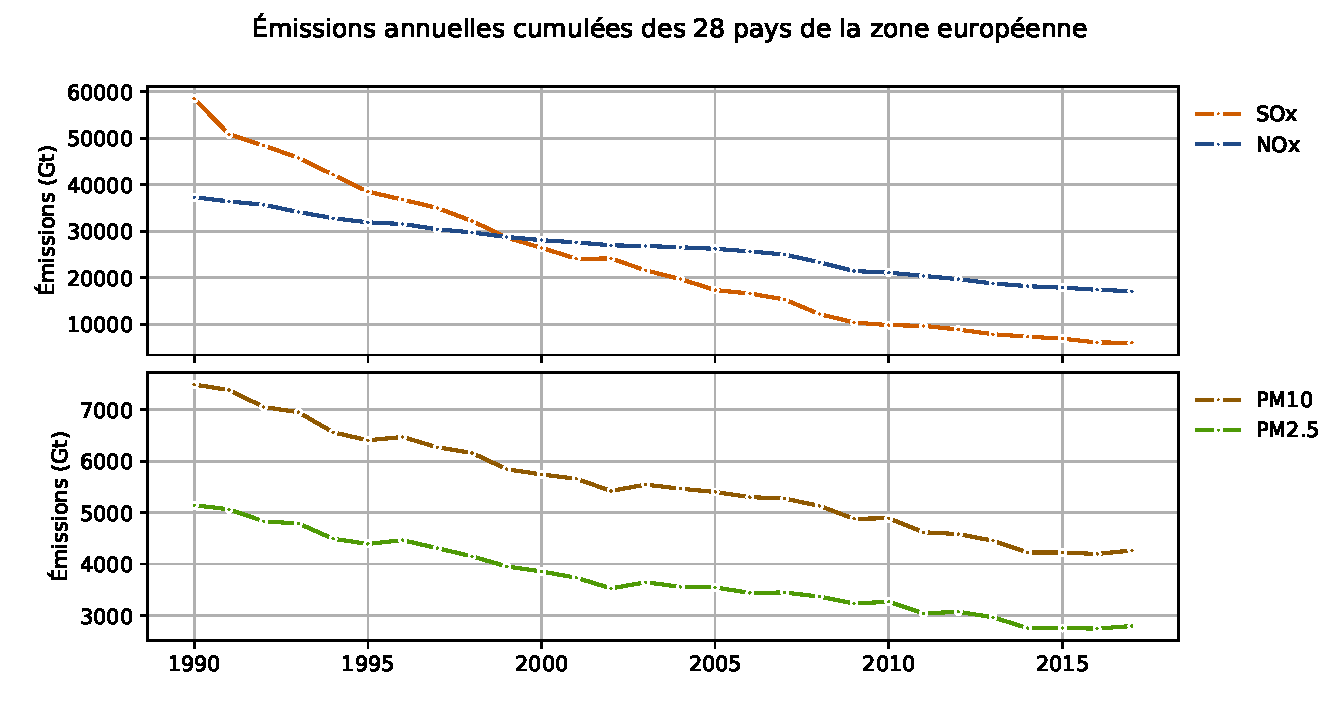
\includegraphics[width=0.9\linewidth]{chapter01/tendance_polluants.pdf}
    \caption{Évolution temporelle des émissions cumulés des 28 pays de la zone européenne
    depuis 1990, indiquant une prise de conscience et une diminution des émissions de
différents polluants gazeux (SOx et NOx) et particulaires (\PMdix{} et \PMdc). Données
issues de \textit{National emissions reported to the Convention on Long-range
Transboundary Air Pollution (LRTAP Convention)}, ©European Environment Agency (EEA).}%
\label{fig:chapter01/tendance_polluants}
\end{figure}


Cependant, la qualité de l'air (incluant les aérosols, mais également les
composés gazeux comme les \ce{NO_x} ou l'ozone) demeure actuellement la 5\ieme{} cause de
mortalité dans le monde, représente un décés sur dix et est catégorisé "cancérogène
certain" par le CIRC depuis 2013. En Europe, pour l'année 2013, c'est
ainsi \num{800000} personne qui sont décédés des suites de maladies cardiovasculaires,
cancer, pneumonie… directement attribuable à la qualité de l'air
\autocite{worldhealthorganizationAmbient2016}. Récemment, \textcite{lelieveldLoss2020}
estiment qu'en moyenne et à travers le monde, c'est 2.9 ans de vie perdue par personne
qui sont imputables à la pollution de l'air, dont 1.7 ans "évitables" car provenant
directement de sources anthropiques.

En termes de bilan financier, la banque mondiale en collaboration avec l'Institute for
Health Metrics and Evaluation (IHME) de l'université de Washington estimait que le coût
associé aux décés prématurés de la seule année 2013 s'évaluait à plus de \$5.11 trillions
de dollar dans le monde~\autocite{worldbankCost2016}.

Afin de limiter cet impact sanitaire, de nombreux pays ont définis des seuils de
concentrations de différents composés (voir Tableau~\ref{tab:seuil_PM} pour les PM).
Seulement ces seuils sont différents d'une institution à une autre. Par exemple, entre
2015 et 2017, le seuil de concentration journalière recommandé pour les \PMdix{} par
l'union européenne (\SI{50}{\ugm} en moyenne journalière) était dépassé pour entre 13 et
19~\% de la population européenne, mais cette proportion augmente à entre 42 et 62~\% si
l'on prend en compte le seuil recommandé de l'OMS de \SI{20}{\ugm} en moyenne
annuelle~\autocite{europeanenvironmentagencyAir2019}.  De plus, il est à noter qu'il
n'existe pas de seuil à partir duquel l'exposition aux PM est inoffensif.

\begin{table}[ht]
    \begin{ThreePartTable}
        \centering
        \caption{Seuils de concentration de PM recommandés par différents organismes.}
        \label{tab:seuil_PM}
        \begin{tabular}{ccSc}
            \toprule
            Organisme       & Polluant & {Concentration (\si{\ugm})} & Période \\
            \midrule
            OMS\tnote{a}    & \PMdc  & 10 & moyenne annuelle       \\
            OMS\tnote{a}    & \PMdc  & 25 & moyenne sur \SI{24}{h} \\
            OMS\tnote{a}    & \PMdix & 20 & moyenne annuelle       \\
            OMS\tnote{a}    & \PMdix & 50 & moyenne sur \SI{24}{h} \\
            Europe\tnote{b} & \PMdc  & 25 & moyenne annuelle       \\
            Europe\tnote{b} & \PMdc  & 20 & moyenne sur 3 ans      \\
            Europe\tnote{b} & \PMdix & 40 & moyenne annuelle       \\
            Europe\tnote{b} & \PMdix & 50 & moyenne sur \SI{24}{h} \\
            France\tnote{c} & \PMdc  & 25 & moyenne annuelle \\
            France\tnote{c} & \PMdix & 50 & moyenne sur \SI{24}{h} (\SI{<35}{jour\per an}) \\
            France\tnote{c} & \PMdix & 40 & moyenne annuelle \\
            \bottomrule
        \end{tabular}
        \begin{tablenotes}
        \item[a] OMS air quality guideline \cite{worldhealthorganizationWHO2006}
        \item[b] Directive 2008/50/EC \cite{officialjournaloftheeuropeanunionDirective2008}
        \end{tablenotes}
    \end{ThreePartTable}
\end{table}

\section{Détermination des sources d'émission des PM}%
\label{sec:source_apportionment_of_pm}

Comme nous l'avons vu, les sources d'aérosols sont très diverses.
Afin de pouvoir avoir un impact sur les concentrations de polluants, il est primordial de
retracer leur provenance. Plusieurs techniques d'analyses existe, qu'elles soient purement
physiques ou géochimiques.

\subsection{Modèle d'attribution des sources}%
\label{sec:source_apportionment_model}

Afin d'estimer la contribution de chaque sources de PM à un point donnée, il est possible
d'utiliser 2 grandes familles de modèles d'attribution des sources (\textit{source
apportionment} (SA)). La première est fondée sur notre connaissance des
émissions et de la météorologie et calcul les réactions physico-chimiques depuis les
sources jusqu'au lieu d'étude (modèle dit de chimie-transport (\textit{chemical transport
model} (CTM)) alors que la deuxième s'évertue à mesurer en un point donné
la chimie des PM et par traitement statistique, attribue à différentes sources ou
''facteurs'' leurs contributions aux concentrations observées (modèle dit récepteur
(\textit{receptor model} RM)).

\subsubsection{Modèle déterministe de chimie-transport}%
\label{ssub:modele_deterministe_de_chimietransport}

\paragraph{Présentation}%
\label{par:presentation}

Les modèles déterministes s'appuient sur l'inventaire des sources d'émissions sur la
région étudiée. Ces cadastres d'émissions sont regroupés en catégorie \textit{Selected
Nomenclature for reporting of Air Pollutants} (SNAP) représentant chacune un secteur
d'activité : Énergie, Procédés industriel, Agriculture, Déchets, Autres et enfin
Naturelle.
Chacune de ces catégories possèdant évidemment des sous-catégories raffinant la
classification (par exemple, les émissions de l'aviation civile de plus de \SI{100}{m} de
long se retrouvent dans le SNAP 080503 (ou \textit{Nomenclature For Reporting} (NFR)
1.3.A.c) autrement dit Énergie - Combustion - Aviation - Aviation civile de plus de
\SI{100}{m})~\autocite{europeanenvironmentagencyEMEP2019}.
À chacun de ces SNAP est associé un profile d'émission (\ce{O3}, \ce{SO2}, NOx, \ce{NH3}, \PMdix, \PMdc,
VOC principalement), obtenu soit par mesure directe, soit par calcul.

Vient ensuite un inventaire de ces sources d'émissions sous forme de cadastre géographique
et temporelle. Notamment la \textit{Convention on Long-Range Transboundary Air
Pollution} (LRTAP) implémenté par l'\textit{European Monitoring and Evaluation Program}
(EMEP) sous l'égide de \textit{United Nations Economic Commission for Europe} (UNECE),
prévoit que les différentes parties prenante à cette convention présentent un rapport de
leurs émissions régulièrement à l'EMEP.

Il est alors possible de construire des modèles déterministes de dispersion et de
réaction des polluants, en couplant un modèle de diffusion résolvant les équations de la
physique de l'atmosphère (navier-stoke, turbulence, rayonnement, etc) avec un modèle
physico-chimique faisant évoluer les composés gazeux et particulaires, incluant leurs
émissions, dépôts, interaction physico-chimique, etc. Pour n'en citer que quelqu'uns : 
Community Multi-scale Air Quality (CMAQ)\footnote{CMAQ: \url{https://www.epa.gov/cmaq}},
Comprehensive Air Quality Model with Extensions (CAMx)\footnote{CMAx : \url{http://www.camx.com/}},
WRF-Chem\footnote{WRF-chem : \url{https://www2.acom.ucar.edu/wrf-chem}},
Chimère,
LOTOS-EUROS...

La raison de la pluralité de ces modèles provient des différentes paramétrisations
possibles des équations physiques, mais également des choix conceptuels de recherche.

\paragraph{Limitations}%
\label{par:limitations}

Comparaison Chimire-DECOMBIO : \textcite{bessagnetHigh2020}

\paragraph{Source apportionment}%
\label{par:source_apportionment}

Concernant l'attribution des sources, il est possible d'utiliser deux techniques au sein
des CTM:

\begin{enumerate}
    \item Faire une première simulation incluant toutes les sources d'émissions (référence
        ou témoin), puis une deuxième simulation avec une source d'émission en moins. La
        différence reflétant l'impacte de la source supprimée sur les concentrations
        ambiantes ;
    \item Garder en mémoire la provenance de chacunes des espèces chimiques lors des
        schémas réactionnels (technique dite de \textit{source labelling} ou \textit{tagged species}).
\end{enumerate}

Seulement, du fait des nombreux processus non linéaires, la suppression d'une source
d'émission aura des répercussions beaucoup plus complexe que la simple diminution des
concentrations propre à cette source (par exemple, des NOx pourraient ne pas passer en
phase particulaire du fait d'un manque d'ammoniac, ou inversement). La première technique
correspond donc à se demander 
\begin{quote}
    Si les émissions de cette source sont diminuée ou supprimée, quels impacts cela va-t-il
    avoir sur les concentrations finales ?
\end{quote}
alors que la deuxième répond à
\begin{quote}
    Dans la concentration ambiante de PM, à combien s'estime la contribution de cette source
    d'émission ?
\end{quote}
Ce sont bien deux questions différentes avec leurs légitimités propres.
Cette dernière technique a commencé été implémenté plus récemment dans certains
CTM~\autocite{wangDevelopment2009,wagstromDevelopment2008,kranenburgSource2013,brandtContribution2013}
et détaillée dans le rapport de~\textcite{mirceaEuropean2020}. Elle présente également
l'avantage de pouvoir tagguer non seulement les sources des espèces chimiques, mais
également leur provenance géographique, c'est-à-dire leur lieu d'émission.

Cependant l'utilisation des CTM présente certaines limites du fait de leur complexité.
Notamment, il semble illusoire de pouvoir un jour inclure toutes les réactions chimiques
possibles dans les modèles déterministes. Notament, les interactions aérosols/neiges ne
sont pas encore complètement compris ni bien représenté dans ces modèles.

Quand bien même ce serait le cas --car les modèles réactionnels sont de plus en plus
poussées--, il faudrait alors avoir des inventaires d'émissions beaucoup plus complet et
précis temporellement, avec aucune certitude d'un oubli potentiel d'une source non prise
en compte. Par exemple une industrie locale non-encore repertoriée, la sous-estimation de
la contribution d'un écosystème, une consommation de bois de chauffage individuel non
inventorié, etc.

Aussi, la limitation physique des modèles météorologiques se retrouvent dans les CTM. Il
est donc compliqué d'envisager, du fait du coût de calcul et de stockage, une simulation à
\SI{10}{m} de résolution spatiale (ou moins), ce qui serait cependant nécessaire pour
appréhender correctement des phénomènes précis, comme les inversions thermiques des
vallées alpines.

\subsubsection{Modèles récepteurs}%
\label{ssub:model_recepteur}

À l'inverse des CTM, il est possible d'estimer les sources contribuant aux concentrations
ambiantes en un lieu donné sans la moindre information météorologique ou simulation
déterministe. Pour cela, il convient de faire des prélèvements sur le lieu d'étude,
d'analyser la chimie que l'on y trouve et retrouver à l'aide de modèle statistique
les différents profils de source et leurs contributions, traduisible pas l'équation
d'équilibre des masses
\begin{align}
    \label{eq:mass_balance}
    X &= G \cdot F
\end{align}
où $X$ est la matrice de dimension $n\times m$ des observations, $G$ est la matrice des
contributions de taille $n\times p$ et $F$ la matrice des profils de taille $p \times n$,
avec $n$ le nombre d'échantillon, $m$ le nombre de variables chimiques mesurées et $p$ le
nombre de facteur.
Un \textit{facteur} peut être une source d'émission (combustion de biomasse par exemple),
mais également regrouper des espèces chimiques provenant d'un même processus secondaire
(nitrate d'ammonium par exemple).
Il est courrant d'exprimer $X$ en \si{\ugm}, $G$ en \si{\ugm} ou concentration
normalisée~\si{[-]} et $F$ en \si{\micro\g\per\micro\g} ou \si{\ugm}.

Si l'on mesure $X$, ce qui nous intéresse ici est de connaître $G$ et/ou $F$.
Si l'on admet que l'on connait a priori les profils d'émissions possibles, alors $F$ est
connue et l'on cherche à estimer $G$. Le modèle de déconvolution adapté est alors le
\textit{Chemical Mass Balance} (CMB). À l'opposé, on peut n'avoir aucune information a
priori à la fois sur les contributions et les profils d'émissions. On utilisera alors le
modèle de déconvolution \textit{Positive Matrix Factorization} (PMF).

Ces 2 types de modèles statistiques sont aux deux extrêmes d'un spectre de modèle de
déconvolution depuis une information ``absolue'' des profils de sources à une absence
totale d'information de ces mêmes profils.  Il existe cependant un continuum entre ces
deux pôles (voir Figure~\ref{fig:chapter01/source_apportionment_methods}), et de nombreux
modèles ont été développés et améliorés depuis la première étude de SA de
\textcite{colucciAutomotive1965} utilisant la ``simple'' corrélation entre le \ce{CO} et
le plomb et benzo(a)pyrène.  Une revue détaillée et historique du fonctionnement de ces
différents modèles peut-être retrouvées dans les articles de
\textcite{henryHistory1997,vianaSource2008,belisCritical2013,hopkeReview2016}.

\begin{figure}[ht]
    \centering
    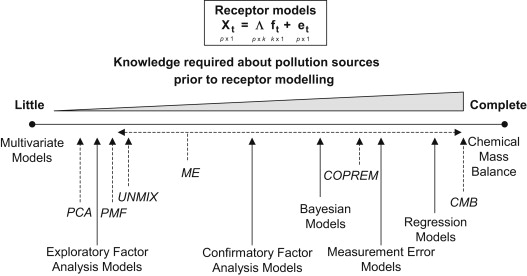
\includegraphics[width=0.7\linewidth]{chapter01/source_apportionment_methods.png}
    \caption{
        Connaissance a priori nécessaire pour les différents modèles de SA existant,
        depuis la simple analyse de facteur par ACP au modèle CMB. Crédit :
        \textcite{vianaSource2008} adaptée de \textcite{schauerCharacterization2006}
    }%
    \label{fig:chapter01/source_apportionment_methods}
\end{figure}

\subsubsection{Chemical mass balance CMB}%
\label{ssub:chemical_mass_balance_cmb}

Le principe du CMB est de déterminer la contribution $G$ d'un nombre de source
aux profils chimiques $F$ prédéfinis aux concentrations ambiantes $X$. Il est donc
nécesaire de connaître les signatures chimiques des sources utilisées.

Afin d'utiliser le modèle CMB --mais également pour d'autres buts-- l'US EPA construit
depuis 1988 la base de donnée SPECIATE~\autocite{simonDevelopment2010}, répertoriant
différents profils d'émission, dont la 5\ieme{}
version a été publié en 2019~\autocite{u.s.environmentalprotectionagencySPECIATE2019}.
Seulement, ces profils sont repésentatifs des sources présentent aux États-Unis et sont
très certainements non transposable à d'autres régions du monde.
En europe, il existe depuis 2016 une base de donnée similaire,
SPECIEUROPE~\autocite{pernigottiSPECIEUROPE2016}, compilant des mesures à l'émission et
d'autres types d'étude permettant d'estimer la signature chimique des profils d'émission.

Cependant, des erreurs ou variabilités locales spécifiques au site recepteur sur ces
profils peuvent conduire à une estimation erronée des contributions finales des
différentes sources.
Aussi, il est necessaire de choisir ou d'aggréger certains des >3000 profils de sources
différents répertoriés afin de restreindre à une valeure réaliste le nombre de sources
potentielle en un lieu donné.
Enfin, les processus secondaires sont mal pris en compte dans ce modèle. L'exemple typique
concerne l'aérosols inorganique secondaire sulfaté, représenté comme un mélange de sulfate
et d'ammonium. Or ce facteur secondaire est souvent associé en réalité à de la matière
organique ou d'autres espèces sulfatées.

\subsubsection{Positive Matrix Factor PMF}%
\label{ssub:pmf}

Un modèle beaucoup plus agnostique que le CMB pour résoudre l'équation de conservation de
la masse a été développé par~\textcite{paateroPositive1994}. Dans cette formulation,
seule la matrice d'observation $X$ est connue, et les matrices de contribution $G$ et des
profils chimiques $F$ sont inconnues.

\paragraph{Formulation mathématique}%
\label{par:formulation_mathématique}

Le principe de la PMF provient initialement de la recherche sur le \textit{machine
learning}, et plus particulièrement de l'analyse factorielle appliqué au problème
bilinéaire $X=G\times F$. L'intérêt initial étant de permettre une réduction
dimensionnelle sans perte d'information. Par exemple, en informatique, une image de $n$
par $m$ pixels forme une matrice $n\times m$ éléments. S'il est possible de retrouver
cette matrice par multiplication de 2 matrices $G$ ($n\times p$) et $F$ ($p \times m$),
alors la quantité d'information stockée dans $G$ et $F$ est $n
\times p + p \times m = p \times (n + m)$. Ainsi, tant que $p < \frac{n\times m}{n+m}$,
alors le nombre d'éléments de $G\times F$ est toujours inférieur au nombre d'élément de
$X$, permettant un gain de mémoire de plus en plus important au fur et à mesure que $n$ et
$m$ augmente.
Tout le problème réside en le fait de trouver la décomposition de $X$ en minimisant
l'erreure engendrée par cette simplification.

Aussi, on observe que la formulation $X = G\cdot F$ est similaire à celle de
la conservation de la masse (Eq.~\ref{eq:mass_balance}). Ce problème peut-être résolu par
analyse en composante principale (ACP), seulement, le résultat obtenu présente des
combinaisons linéaire (additive et soustractive) des différents composants. Cette possible
négativité des composants n'a pas de sens dans beaucoup de domaine physique, y compris en
géochimie. \textcite{paateroPositive1994} présente donc une nouvelle méthode de
déconvolution, implémentant une contrainte de non-négativité, nommée \textit{Positive Matrix
Factorization} (PMF). 

La formulation est la suivante : étant donné une matrice d'obervation $X$ de taille
$n\times m$, une matrice associée des incertitudes $U$ de taille $n \times m$ et un rang
$p$, alors 
\begin{align}
    \label{eq:pmf_formulation}
    X &= G \cdot F + E \\
    \forall i,k,j &, G_{ik}\geq 0 \text{ et } F_{kj}\geq 0\\
    Q &= \sum_{i=1}^n\sum_{j=1}^m E_{ij}^2/U_{ij}^2\\
    {Q, F} &= \argmin_{G,F} Q.
\end{align}

Différent algorithme de résolution du système Eq.~\ref{eq:pmf_formulation} ont été développés.
L'implémentation initiale de~\textcite{paateroLeast1997} a été amélioré pour pouvoir
ajouter des contraintes sur les matrices $G$ et $F$, notamment grâce au solveur
\textit{multi-linear engine} (ME-2) \autocite{paateroMultilinear1999}. En effet, il
n'existe pas de solution unique au problème Eq.~\ref{eq:pmf_formulation}, notamment, car le
système est invariant par rotation:
\begin{align}
    \label{eq:rotationalambiguity}
    X   &= G \cdot F + E \\
        &= (G \cdot T) \cdot (T^{-1} \cdot F) + E\\
        &= G' \cdot F' + E
\end{align}
et ainsi une infinité de solution coexistent. 

\paragraph{Interprétabilité du modèle PMF}%
\label{par:interpretabilite_du_model_PMF}

L'avantage de la PMF réside en le fait que l'algorithme n'est pas fondé sur la
correlation entre variable, comme c'est le cas de l'ACP, mais bien en la formation d'un
modèle additif linéaire de ce qui est observé.
\begin{quote}
    We shall not be satisfied in finding some correlations, we wish to form a quantitative
    model of what was observed! \autocite{paateroPositive1994}
\end{quote}

Il a été montré que la PMF est capable d'extraire des informations partielles cohérentes des
données là où l'ACP n'est qu'une représentation holistique~\autocite{leeLearning1999}. Par
exemple, appliquée à la reconnaissance d'image faciale, la PMF déconvolu les visages en
sous partie (bouche, sourcils, front, etc) alors que d'autres méthodes ''se contentent''
d'une approche globale de l'information et où seules les premières dimensions portent
l'information nécessaire à la reconstruction du signale (voir
figure~\ref{fig:chapter01/NMFvsPCA}).

\begin{figure}[ht]
    \centering
    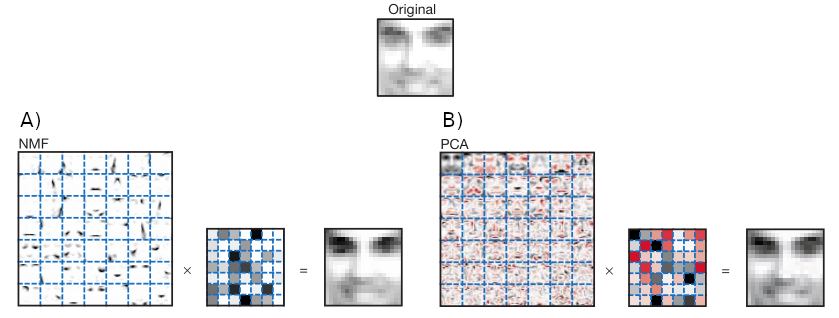
\includegraphics[width=1.0\linewidth]{chapter01/NMFvsPCA.png}
    \caption{Analyse factorielle par PMF (i.e. NMF for \textit{non-negative matrix
    factorization}) et ACP d'une banque d'image de 2429 images en niveau de gris de 19
    pixel par 19 pixels. Les deux techniques essaient de reproduire l'image originale en
    fonction de leur apprentissage.
    \textbf{A)} Le rang de la PMF est $p=49$, correspondant aux 49
    représentations des $19\times19$ images à gauche, chacune étant un facteur de la
    matrice $F$, et leurs ''contributions'' respectivement identifiées par le carré de 7 par
    7 en niveau de gris, à droite.
    \textbf{B)} Analyse en composante principale, le carré de gauche représentant les 49
    vecteur propres et celui de droite les 49 valeurs propres.
    Les échelles de couleurs sont : rouges pour les coefficients négatifs, noirs pour les
    coefficients positifs.
    Figure adaptée de \textcite{leeLearning1999}}%
    \label{fig:chapter01/NMFvsPCA}
\end{figure}

\paragraph{Applicabilité en science de l'atmosphère}%
\label{par:applicabilité_en_science_de_l_atmosphère}

Dans le cas qui nous intéresse ici, cela signifie que chacun des vecteurs de la matrice
$F$ correspond à un profil chimique, en \si{\ugm}, indépendant des autres profils, et
que la matrice $G$ représente la contribution de chacun de ces profils au jour
considéré, de manière cohérente avec l'équation de conservation de la masse.

Puisque la PMF ne nous donne qu'un profil chimique, certains de ces profils représentent
directement une source d'émission, et d'autres correspondent à un ensemble de processus
conduisant à un profil chimique stable. On ne peut donc pas appeller ``source'' tous les ensembles
identifiés par la PMF puisque certains ne sont pas à proprement parler émient tel quel et
proviennent de processus physico-chimique ayant eu lieu après les émissions de ces
composés.
Le terme de \textbf{facteur} est donc utilisé pour désigner un profil chimique et sa
contribution.

L'application du modèle PMF a été utilisé de nombreuse fois, et a été grandement favorisé
par son implémentation dans le logiciel de l'EPA: EPA PMF5.0~\autocite{norrisEPA2014}.
Si l'EPAPMF5 est massivement utilisé pour les données provenant d'analyse de
filtre, l'utilisation de spectre de masse provenant de mesure d'AMS est facilité par
l'utilisation du logiciel SoFi~\autocite{canonacoSoFi2013}. Ces deux logiciels utilisent
le solveur ME-2 pour résoudre le système d'équation de la PMF.

\paragraph{Estimation des incertitudes}%
\label{par:incertitudes}

Il existe différent type d'incertitude pour ce modèle : 1) la sensibilité aux données
d'entrée (sur ou sous représentation de certains événements : impact d'un point
``extrème'' par exemple) et 2) l'incertitude rotationelle~\autocite{brownMethods2015}.

La première incertitude est évaluée à travers une méthode de \textit{bootstrap} consistant
à rééchantilloner par block la matrice des observations $X$, à reconduire une simulation
PMF et a faire correspondre chacun des nouveaux facteurs obtenus à ceux qui leur sont le
plus proches dans la simulation initale.
On obtient ainsi une incertitudes sur les profils chimiques mais également sur les
contributions temporelles.
Cela permet aussi d'évaluer si la solution initale était statistiquement peu fréquente
dans l'espace des possibles ou si au contraire elle correspond à minimum de la fonction
coût $Q$ relativement commun.

L'incertitude rotationelle s'estime par méthode dite de \textit{displacment}. La gamme des
valeurs possibles de chacune des espèces chimiques de chacun des profiles correspondant à
une variation de la fonction coût $Q$ inférieur à une quantité donnée (par exemple $dQ =
0.5\%$) est évaluée. Toutes ces valeurs sont alors possibles, et correspondent donc à
l'incertitude rotationelle de la solution.

\paragraph{Limitation de l'ambiguité et contrainte géochimique}%
\label{par:limitation_de_l_ambiguité_et_contrainte_géochimique}

Cependant, il est possible de limiter l'ambiguité rotationelle et donc de limité
l'incertitude de la solution par l'ajout de contrainte géochimique au modèle statistique.
Cela est rendu possible par le solver ME-2 qui permet notamment l'ajout de contraintes
sur les matrices $G$ et $F$, limitant de fait le nombre de rotation possible de ces
matrices. Ce faisant, l'utilisateur rajoute de la connaissance a priori au modèle qui
était jusqu'alors purement statistique. C'est pourquoi dans la
figure~\ref{fig:chapter01/source_apportionment_methods} le ME-2 n'est pas à l'extrèmité de
l'axe : l'utilisateur rajoute de la connaissance sur les profils ou contributions
temporelles des différents facteurs.

L'ajout de ces contraintes limites de fait les rotations possibles des matrices $F$ et
$G$, conduisant non-seulement à des solutions géochimiquement plus compréhensibles mais
aussi à une incertitude plus faible des profils des différents facteurs.

\paragraph{Subjectivité de l'expérimentateur}%
\label{par:subjectivité_de_l_expérimentateur}

L'utilisateur a donc 3 paramètres à choisir manuellement : les observations $X$, leurs
incertitudes $U$ et le nombre de facteur (ou rang) $p$. Chacuns de ces paramètres
influencera la solution finale obtenue et provient de la subjectivité de l'expérimentateur:
quelles espèces chimiques utiliser ? garder ou non ce jour d'observation ''extrême'' ?
quelles incertitudes pour quelles espèces ? combien de facteur utiliser ?

Une inter-comparaison de modèle récepteur sur le site de Lens a été conduit par
\textcite{belisEvaluation2020}. Les 38 études des participants bénéficiaient de
la même base de donnée et non seulement le nombre de facteur retrouvé varie de 5 à 12 mais 
le contributions temporelles, bien que globalement concordante, varient entre les
différentes études, comme le montre les z-scores de la figure~\ref{fig:chapter01/belisEvaluation2020_fig2a}
\footnote{Le z-score représente ici une distance entre les contributions temporelles de
    chacune des sources des différentes études à la moyenne de celles-ci, définie par 
    \begin{align}
        \label{eq:z-score}
        z = \frac{x-X}{\sigma}
    \end{align}
    où $x$ est une série temporelle d'un facteur, $X$ la moyenne des séries temporelles de
    ce facteur issue des différentes études et $\sigma$ définie comme $0.5\times X$
    \parencite{pernigottiDeltaSA2018}.
}.

Cette diversité s'explique par le \textbf{choix des variables utilisées par la PMF}, reposant au
final sur la ''connaissance d'expert'' de l'expérimentateur. En effet, toutes les données
d'entrée ne portent pas la même quantité information et l'ajout d'espèces traceuses de
sources particulières conduira à l'obtention d'un facteur relié à cette source. Au
contraire, l'ajout trop important d'espèce n'apportant pas suffisamment d'information peut
déstabiliser statistiquement le modèle et résulter en une solution statistiquement faible
(peu de répétabilité, variance importante, etc) et de fait géo-chimiquement douteuse.
Aussi, le \textbf{choix des contraintes} à appliquer impliquera des solutions
nécessairement différentes. Là encore, ces contraintes sont issues de la connaissance a
priori de l'expérimentateur et sont donc en partie subjective.

Enfin, l'identification des facteurs est laissé à l'appréciation de l'expérimentateur. Il
faut donc savoir identifier quel profil d'émission peut être responsable du facteur
observé. Cette nomenclature des facteurs est elle aussi subjectif et non standardisée :
véhiculaire, émission routière, trafic routier, combustion diesel, etc. peuvent être
différents noms donnés au même profil, par différents utilisateurs.
% Des travaux récents, portés par le groupe FAIRMODE du JRC, portent notamment sur une
% harmonisation de cette nomenclature, à travers la construction d'une donnée européenne de
% profil de source standardisée et hierarchisé : SPECIEUROPE~\autocite{pernigottiSPECIEUROPE2016}.

Pour toutes ces raisons, la comparabilité des profils issus de différentes études PMF
est donc un sujet en cours de recherche, et sera abordé plus en détail dans le
chapitre~\ref{cha:approfondissement_des_connaissances_des_sources_des_pm}.

\begin{figure}[ht]
    \centering
    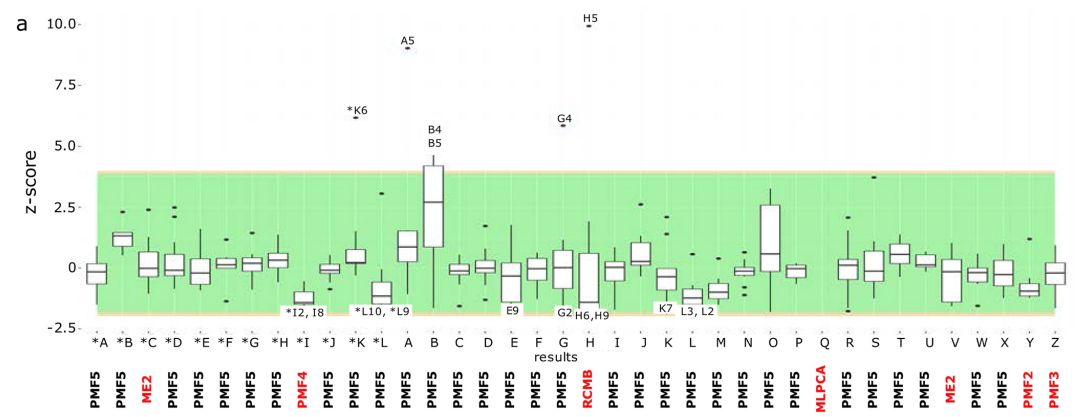
\includegraphics[width=1.0\linewidth]{chapter01/belisEvaluation2020_fig2a.png}
    \caption{Comparabilité des séries temporelles obtenues par les 38 différentes solutions
    sur l'étude de comparaison des modèles sources-récepteurs sur le site de Lens par
    rapport à la moyenne de l'ensemble des différentes études. L'axe X représente chacune des
    solutions des participants, et l'axe Y le z-score, mesure de la similitude des
contributions temporelles. Source: \textcite{belisEvaluation2020}}%
    \label{fig:chapter01/belisEvaluation2020_fig2a}
\end{figure}

\subsection{Atouts et limitations des différents modèles récepteurs}%
\label{ssub:atouts_et_limitations_des_différents_modèles_récepteurs}

Les 3 types de modèles listés précedemments (CTM, CMB et PMF) ne sont pas les seuls
utilisés, mais représentent néanmoins la très grandes majorités des études d'attribution
des sources. Leurs atouts et limitations sont repris dans le
tableau~\ref{tab:comparison_SA} et nous expliqueront dans cette partie plus en avant le
choix du modèle PMF avec analyse chimique sur filtre pour cette thèse.

\subsubsection{La PMF : modèle théoriquement le moins biaisé par l'information a priori}%
\label{ssub:choix_du_modèle_pmf}

Lorsque l'on s'intéresse à un site particulier, le contexte géographique peut nous donner
des indications sur les sources majoritaires. Seulement, prédéfinir à l'avance les sources
possibles résulte en un biai évident : on ne voit que ce que l'on s'attend à voir.
L'utilisation des CTM ou du CMB ne nous permet donc pas de découvrir de nouvelles sources
locales. Au mieux, le modèle échoueron à reproduire les observations, ce qui indiquerai
une source ou un processus manquant.

Au contraire, la PMF étant totalement agnostique aux sources ou processus réels, les
facteurs déterminés reflète les observations locales sans biai. Ainsi, l'ajout d'une
espèce peut conduire à découvrir et quantifier une nouvelle source d'émission ou processus
atmosphérique, jusqu'alors non prise en compte ou sous-estimée, comme nous le verrons dans
le chapitre~\ref{cha:approfondissement_des_connaissances_des_sources_des_pm}. À noter
également que la réciproque est vrai : la non-prise en compte d'une espèce chimique peut
conduire à ne pas identifier un facteur important, ayant un impact directe sur la
contribution des autres facteurs aux PM.
Toute la difficulté réside dans le choix des ``bonnes espèces'' et en l'interprétation de
ce modèle, fondé sur nos connaissances géochimiques.

\subsubsection{Analyses chimiques ou spectroscopie de masse}%
\label{ssub:analyses_chimiques_ou_spectroscopie_de_masse}

Comme expliqué précédemment, les PM sont composés en grande majorités de matière organique
--tout du moins dans les écosystèmes européens.  Devant la myriade d'espèce chimique la
constituant, la caractérisation exhaustive de cette matière organique est illusoire.
Pourtant, il est possible de décrire cette matière organique de manière extrèmement
précise par spectroscopie de masse (\textit{aerosol mass spectrometer} (AMS)). On obtient alors des
fragments d'espèces chimiques ionisées, caractérisés par leur ratio masse sur charge ionique
($m/z$ ou Th).

L'avantage principale est la quasi exhaustivité et la posibilité de
résolution temporelle fine pouvant aller à un échantillon toutes les 2 minutes
\autocite{marmureanuOnline2020}.  Le désavantage majeure est la quantité extrèmement
importante de données générées à analyser. En plus, l'identification des fragments en
facteur PMF est difficilement interprétable en terme de source d'émission. En effet, si
l'on retrouve des facteurs primaires comme l'\textit{hydrocarbon-like organic} (HOA)
pouvant être relié au trafic ou le \textit{biomass burning organic aerosol} (BBOA),
certains, reflétant des processus secondaires, sont plus ``abstrait'' et classé selon leur
degrée d'oxygénation : \textit{less-oxidized oxygenated organic aerosol} (LO-OOA) ou
encore \textit{more-oxidized oxygenated organic aerosol} (MO-OOA).
Enfin, l'utilisation de PMF sur données AMS présente aussi la limitation de ne prendre en
compte que la matière organique. Il est donc difficile voir impossible d'estimer la
contribution des poussières crustal, présentant très peu ou pas de matière organique. De
même, les émissions secondaires du trafic comme l'usure des freins ou des pneu ne peuvent
pas être retrouvées par PMF-AMS.

Les méthodes de PMF-AMS sont cependant récente et en développement très rapide et ces
dernières années nouveaux travaux tentent de combiner mesure AMS et mesure chimique sur
filtre~\autocite{vlachouAdvanced2018,vlachouDevelopment2019}.  Cependant, lorsque l'on
s'intéresse aux sources d'émissions dans une optique réglementaire et non de compréhension
fine des processus secondaires, la PMF avec analyse chimique sur filtre reste pour
l'instant d'avantage adaptée que la PMF-AMS.

En effet, les analyses sur filtres permettent l'identification des types d'espèces
chimiques plus large qu'uniquement la matière organique (ions et métaux notamment).  Le
recul scientifique des analyses chimiques sur filtres est également appréciable pour
déterminer les sources ou processus à l'œuvre.

Enfin, et plus spécifiquement à cette thèse, nous chercherons à analyser d'autres
variables que la chimie (notament le potentiel oxydant, voir
section~\ref{sec:le_potentiel_oxydant_des_aerosols}) sur les mêmes échantillons que les
mesures de chimie. Cela exclut donc les données AMS on-line et donc la résolution
temporelle fine, réduisant l'intérêt de cette methode pour cette thèse.

\begin{table}[!ht]
    \begin{ThreePartTable}
        \centering
        \caption{Forces et limitations des différents modèles d'attribution des sources}
        \label{tab:comparison_SA}
        \footnotesize
        \begin{tabular}{cp{0.43\textwidth}p{0.43\textwidth}}
        \toprule
        Type & Atouts & Limitations \\
        \midrule
        CTM &
        \begin{itemize}[topsep=0pt, left=0pt, label={\unicodesymbols ✔}]
          \item Grande couverture spatiale et temporelle
          \item Comparaison facilité : sources identiques partout\tnote{a}
          \item Prévision à court et long terme
          \item[{\unicodesymbols ~}] Peu de subjectivité\tnote{b}
        \end{itemize}
            &
        \begin{itemize}[topsep=0pt, left=0pt, label={\unicodesymbols ✘}]
          \item Nécessite des cadastres d'émissions
          \item Nécessite un modèle météo
          \item Ne voit que ce qui est donnée des cadastres
          \item Variabilité temporelle des émissions peu robuste
          \item Nombre d'espèces chimiques limités
        \end{itemize}
        \\ \midrule
        CMB & 
        \begin{itemize}[topsep=0pt, left=0pt, label={\unicodesymbols ✔}]
          \item Spécificité du site potentiellement prise en compte
          \item Grand nombre d'espèces pouvant être utilisé
        \end{itemize}
            & 
        \begin{itemize}[topsep=0pt, left=0pt, label={\unicodesymbols ✘}]
          \item Faible représentativité spatiale et temporelle
          \item Prélèvement et analyses couteux (humain et financier)
          \item Profils des sources fixes et connu à l'avance
          \item Nécessite une base de connaissance de profils chimique
          \item Subjectivité de l'experimentateur
        \end{itemize}
        \\ \midrule
        PMF &
        \begin{itemize}[topsep=0pt, left=0pt, label={\unicodesymbols ✔}]
          \item Pas besoin de connaissance a priori des sources
          \item Spécificités du site prise en compte
        \end{itemize}
            & 
        \begin{itemize}[topsep=0pt, left=0pt, label={\unicodesymbols ✘}]
          \item Faible représentativité spatiale et temporelle
          \item Prélèvement et analyses couteux (humain et financier)
          \item Nécessite des espèces traceuses
          \item Grand nombre d'échantillon requis
          \item Subjectivité de l'experimentateur
        \end{itemize}
        \\
        PMF-AMS &
        \begin{itemize}[topsep=0pt, left=0pt, label={\unicodesymbols ✔}]
          \item Grande caractérisation de la matière organique
          \item Possibilité de résolution temporelle très fine (mesure on-line)
        \end{itemize}
            & 
        \begin{itemize}[topsep=0pt, left=0pt, label={\unicodesymbols ✘}]
          \item Difficultés d'interprétation
          \item Cible spécifiquement la matière organique
          \item Peu utile pour la réglementation
        \end{itemize}
        \\
        PMF-filtre &
        \begin{itemize}[topsep=0pt, left=0pt, label={\unicodesymbols ✔}]
          \item Large gamme de famille d'espèce chimique
          \item Directement applicable pour la régulation
          \item D'autres analyse possible sur le même filtre (potentiel oxydant par
              exemple)
        \end{itemize}
            & 
        % \begin{itemize}[topsep=0pt, left=0pt, label={\unicodesymbols ✘}]
        % \end{itemize}
        \\
        \bottomrule
        \end{tabular}
    \end{ThreePartTable}
\end{table}


\subsubsection{Nécessité d'inclure des espèces traceuses dans les PMF}%
\label{ssub:nécessité_d_inclure_des_espèces_traceuses}

L'une des limitations des PMF provient de leur sensibilité aux espèces chimiques
utilisées.

\todo{Discussion espèce organique}
\autocite{srivastavaSpeciation2018a}etc

\section{Vers une mesure unifiée de l'impact sanitaire : le potentiel oxydant}%
\label{sec:le_potentiel_oxydant_des_aerosols}

Devant la grande variété de chimie, forme, taille, etc. des aérosols, il apparaît
compliqué de résumer la toxicité de l'air que l'on respire à la simple concentration
massique en aérosols. En effet, il est évident que respirer un~\si{\ugm} de sable n'aura
pas le même impact sur notre santé qu'un~\si{\ugm} de mercure ou de plomb.  Seulement, la
mesure des concentrations est l'une des plus simples à implémenter en routine et est également
facilement automatisable, permettant ainsi un premier ordre de grandeur de l'exposition
des populations. Aussi, il est important de rappeler que les aérosols n'ont pas qu'un
impact sanitaire, mais également climatique ou environnementale (voir
section~\ref{ssub:impacts_climatiques} et~\ref{ssub:impacts_environnementaux}),
pour lesquels la mesure de la concentration est tout à fait adapté.

Bien qu'il ne soit pas encore établi de mécanismes clairs entre le PM et leur impact
sanitaire, leur capacité à induire un stress oxydant dans notre corps est une des
hypothèses privilégiées, notamment par leur transport ou induction d'espèces réactive de
l'oxygène (\textit{reactive oxygen species}
(ROS))~\autocite{squadritoQuinoid2001,liParticulate2003a,liUltrafine2003,gonzalez-flechaOxidant2004}.

La présence de ROS dans nos cellules est un phénomène naturel, produit en grande partie
par catabolisme oxydatif et notamment la respiration cellulaire lors du transfert
d'électron depuis le \ce{O2} vers l'accepteur final \ce{H20}. Lors de ce transfert, il est
possible d'avoir des électrons captés par d'autres espèces chimiques, conduisant à la
formation de l'anion superoxyde \ce{O2^{.-}} ou \ce{HO^{.-}}, entre autres.
En temps normal, les anti-oxydants cellulaires réduisent ces oxydants avant qu'ils ne
puissent avoir des effets délétères sur les chaînes protéïques ou les acides nucléiques.

Seulement, au contact de nos poumons, les PM, oxydantes, interagissent donc avec nos
anti-oxydants naturels~\autocite{kellyProtein2003}, voir traverse la paroi épithéliale
et entre dans la circulation générale et les cellules internes.
Dans un premier temps, les défenses anti-oxydantes sont mobilisées, puis si l'oxydation se
poursuit, on a alors une inflammation, puis cytotoxicité~\autocite{baezaPollution2007}.

\begin{figure}[ht]
    \centering
    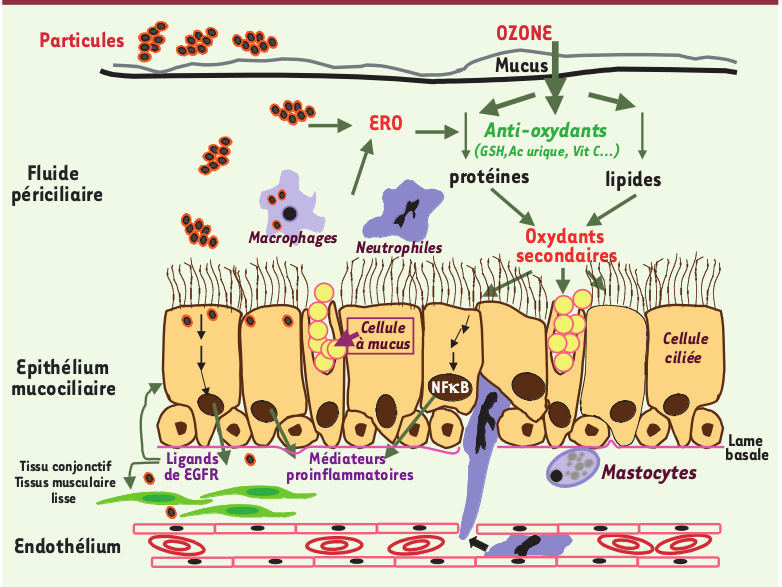
\includegraphics[width=0.8\linewidth]{chapter01/OxydativeMechanism_BaezaMorano2007.png}
    \caption{Mécanismes de toxicité de l’ozone et des particules atmosphériques dans les voies
    aériennes. Crédit : \textcite[figure 1]{baezaPollution2007}}%
    \label{fig:mecanisme_oxydation}
\end{figure}

Afin de répondre à cette problématique de métrique sanitaire des PM, il a été proposé
par~\textcite{zielinskiModeling1999} et \textcite{choRedox2005} une nouvelle mesure,
intégratrice des propriétés physico-chimique des aérosols, sensé être plus proche des
impacts sanitaires occasionés par les PM : le \textit{potentiel oxydant} (PO, ou
\textit{oxidative potential} (OP)).
Cette nouvelle mesure tente de quantifier les espèces réactive de l'oxygène présentent
ou induite par les aérosols par la mise en contact des aérosols avec un anti-oxydant.
Le suivi de la cinétique de la réaction permet ainsi d'estimer la réactivité de la
particule, prenant en compte non seulement sa chimie, mais aussi la taille et forme des
particules à travers leurs surfaces de réaction et également les potentiels ''effet
cocktail'' lors de la combinaison de différentes espèces chimiques.

L'avantage de cette méthode accellulaire est qu'elle est peu couteuse, non-invasive et
implémentable en routine en laboratoire, comparativement aux tests cellulaires nécessitant
des prélèvements de tissu et analyse des protéines marqueuses de l'inflammation.
Elle permet également une confrontation facilitée aux autres informations dont l'on dispose
sur les PM provenant du même échantillon.

\subsection{Methodologie de mesure}%
\label{sub:methodologie_de_mesure}

Il n'existe pas à l'heure actuelle de méthodologie standardisée de mesure du potentiel
oxydant. Plusieurs méthodes coexistent et apportent chacune une vision différente du PO.

Il faut noter également que ces méthodes n'ont pas été développées lors de ma thèse mais
s'appuient sur les travaux de \textcite{calasPollution2017} et que les échantillons ont été
analysés par les différents techniciens et techniciennes du plateau analytique Air-O-Sol.

\subsubsection{Différents agents réactants}%
\label{ssub:differents_agent_reactant}

La mesure du PO se faisant par suivi cinétique de la déplétion d'un anti-oxydant
lorsqu'il est mis au contact des PM, le choix dans l'anti-oxydant induit des mesures de PO
différentes. Au cours de cette thèse, 2 mesures différentes sont utilisées conjointement :
le test au dithiothreitol (DTT) et à l'acide ascorbique ou vitamine-A (AA), et sont
explicités dans le chaptire suivant (section~\ref{sub:potentiels_oxydants}).

D'autres méthodes de mesures du PO existent, mais n'ont pas été utilisées au courant de
cette thèse, à savoir :
\begin{description}
    \item[Electron spin resonance ESR] sensé ciblé particuliairement le radical
        \ce{HO^{.}} \autocite{shiHydroxyl2003,shiTemporal2003}
    \item[DCFH]\todo{ref}
    \item[Mélange d'anti-oxydant] Bien que la plupart du temps testé indépendament, il est
        possible d'estimer un ''PO moyen'' par la mise en contact de différents
        anti-oxydants simultanément (acide ascorbique, glutation et urée par exemple)~\autocite{calasComparison2018}
\end{description}

\subsubsection{Un ''meilleur'' test que les autres ?}%
\label{ssub:un_meilleur_test_que_les_autres_}

Les différents tests de PO ne sont pas sensibles aux mêmes espèces chimiques ni même aux même
conditions physico-chimiques. En effet, l'étude de \textcite{kunzliComparison2006} sur 20
sites européens présente des corrélations différentes entre le PO mesuré par ESR, AA ou
GSH au regard de la masse des PM et les métaux les constituants.
Ce résultat a été retrouvé depuis par de nombreuses études, et pour le test au DTT et DCFH
également. Par conséquent, cela montre que différents constituants des PM agissent
différemment et à travers des mécanismes oxydatifs divers, capturés par certains tests et
non par d'autres.
Il est donc probable que certaines affections sanitaires soient relié à un test donné, et
d'autre affection à un autre test. En l'absence de travaux plus approfondis en toxicologie
et épidémiologie, il n'est donc pas possible en l'état actuel des connaissances de trancher
pour ''le meilleur test de PO''.

Par conséquent, les travaux de cette thèse s'emploient à étudier le PO mesuré par DTT et
par acide ascorbique conjointement.


\subsection{Attribution du PO aux sources d'émissions des PM}%
\label{sub:attribution_du_po_aux_sources_d_émissions_des_pm}

Les mesures de PO étant fastidieuse, il a fallu attendre la mise en place de technique
de semi-automatisation pour obtenir des séries temporelles de mesure de PO. Les récents
travaux de \textcite{fangSemiautomated2015}, parallement aux travaux de
\textcite{calasPollution2017}, ont permis ce pas technique, permettant l'analyse accrue de
prélèvement et les premières séries annuelles de PO, conjointement avec l'analyse de la
chimie des filtres prélevés.

\subsubsection{Corrélation PO - chimie}%
\label{ssub:corrélation_po_chimie}

Les liens entre la chimie des particules et les PO s'est dans un premier temps focalisé
sur la simple corrélation univariée. Ainsi, le Cu présente de forte corrélation
avec le \PODTT{} et \POAA, de même que le carbone organique, etc. Seulement, la simple
corrélation montre également une forte corrélation entre le \PODTT{} et le \ce{NO3-},
pourtant inerte en termes d'oxydo-réduction.
En effet, une corrélation n'implique pas une causalité, et cette corrélation est en effet
une co-corelation entre le \ce{NO3-} et d'autres espèces, rédox-actives.

\todo{parler des quinones, add ref, etc}


\subsubsection{Sources de PM et de PO}%
\label{ssub:sources_de_pm_et_de_po}

% Enfin, il n'est pas possible de mesurer l'ensemble des espèces chimiques constituant les
% PM. Devant cette foultitude, il parait donc illusoire de pouvoir attribuer un PO
% intrinsèque à chacune des espèces chimique.
% En revanche, si l'on bénéficie d'un nombre suffisant d'échantillon, il est alors possible
% d'estimer les sources ou facteurs d'émissions (voir
% section~\ref{sec:source_apportionment_of_pm}). Ce faisant, la vision par ''source'' plutôt
% que par ''espèce'' permet une agrégation de l'information, en regroupant un ensemble
% d'espèce, mesurée ou non, provenant d'une même source d'émission, en une seule variable.
% Ainsi, il est possible d'attribuer un PO à une source donnée, sans pour autant avoir
% besoin de savoir quelles sont les espèces chimiques émises par cette source qui
% contribuent au PO.
% De plus, en termes de régulation, la vision par source est davantage pertinente car permet
% potentiellement une action politique plus rapide que s'il s'agissait de cibler une espèce
% chimique particulière.

Il est aussi possible de chercher à attribuer un PO non pas à une espèce chimique mais à
une source spécifique.
\todo{work in progress}
\paragraph{Mesures directes à l'émission}%
\label{par:mesures_directes_à_l_émission}

\paragraph{Études sur sites et en air ambiant}%
\label{par:études_sur_sites_et_en_air_ambiant}

Les premières études de ce type sont celles de
\textcite{vermaReactive2014,batesReactive2015,fangOxidative2016}, et utilisent 2 approches
différentes :
\begin{enumerate}
    \item Incorporation de PO comme variable d'entrée d'une étude PMF au même titre qu'une
        autre espèce chimique ;
    \item Analyse de sources via le CMB (sans PO), puis régression linéaire entre les
        sources de PM ainsi déduites et le PO.
\end{enumerate}
Bien que de façons inhérente aux différences entre PMF et CMB les sources retrouvées ne
sont pas exactement les mêmes, ils montrent que la combustion de biomasse est la source
principale de \PODTTv, suivit de près par le trafic routier (ensemble des émissions
véhiculaire et de la remise en suspension de poussière de route), puis le sulfate
d'ammonium et enfin un facteur de composés organiques secondaires solubles.
Concernant le \POAAv, \textcite{fangOxidative2016} (voir
figure~\ref{fig:chapter01/fangOxidative2016-fig4}) estiment à autour de 45\% la
provenance véhiculaire et à environ 50\% la contribution de facteur secondaire (organique
et inorganique).

\begin{figure}[ht]
    \centering
    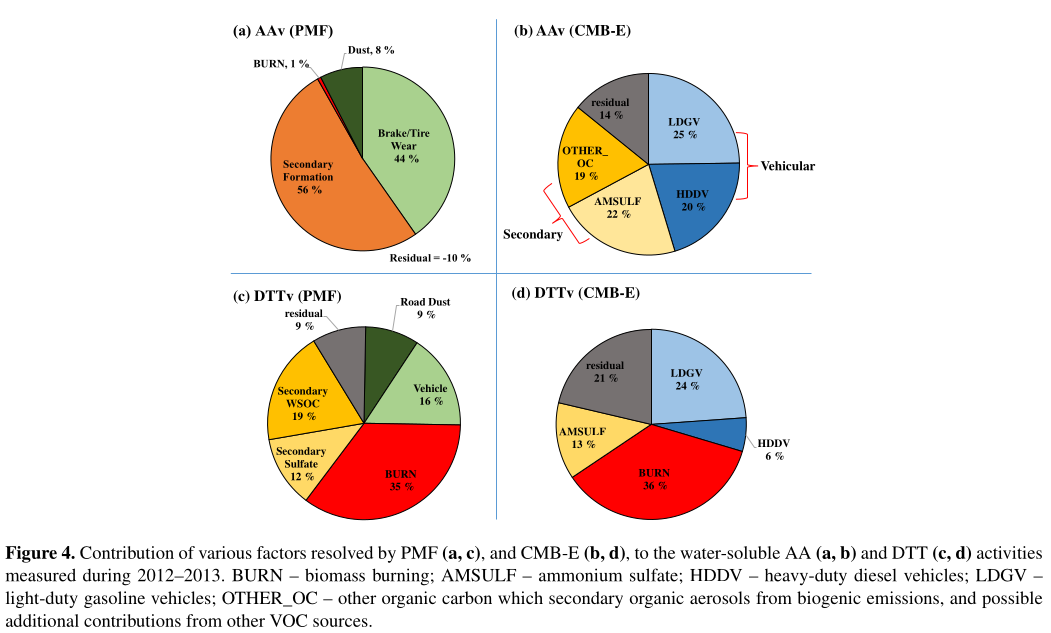
\includegraphics[width=1.0\linewidth]{chapter01/fangOxidative2016-fig4.png}
    \caption{Contribution des sources de PM aux \POAAv{} et \PODTTv{} par l'étude de
    \textcite{fangOxidative2016} portant sur un ensemble de 238 échantillons sur 3 sites
        distincts à Atlanta, US, pendant l'année 2012-2013.}%
    \label{fig:chapter01/fangOxidative2016-fig4}
\end{figure}

Lors du commencement de ma thèse, seules ces études étaient, à ma connaissance,
disponibles dans la littérature concernant l'attribution des sources de PM aux potentiels
oxydants.  Depuis, de nouvelles études ont été publiés, et seront discutés dans le
chapitre~\ref{cha:application_to_15_sites_in_France}.


\section{Objectifs de cette thèse}%
\label{sec:positionnement_de_cette_thèse}

Ma thèse s'inscrit donc dans cette double problématique de l'identification et de la
quantification des contributions massiques des différentes sources d'émission de PM en air
extérieur, mais aussi de leur contribution au nouvel indicateur qu'est le potentiel
oxydant.

Premièrement, il s'agit d'améliorer l'outil de déconvolution des sources de PM
\textit{Positive Matrix Factorization}, non pas par nouveau développement mathématique de
résolution de l'équation de conservation des masses, mais par l'élaboration d'une
expertise dans les différentes paramétrisations de ce modèle, dans son entraînement et
dans la critique de ses résultats. Notamment, la questions de la présence de l'ensemble
des sources majoritaires se posera dans le
chapitre~\ref{cha:approfondissement_des_connaissances_des_sources_des_pm}, à travers
l'implémentation de nouveux traceurs chimiques ou isotopiques.
Également, les incertitudes des solutions PMF ne sont quasiment jamais explicités alors
que c'est une question centrale qui intéressent d'autant plus les décideurs publique. Mes
travaux tenterons donc de quantifier les incertitudes des contributions des sources aux
espèces mesurées.
Aussi, pour pouvoir généraliser des études PMF à différents sites, il faut auparavant
non seulement s'assurer que les méthodes sont similaires entre les études (mêmes espèces
chimiques…) mais aussi estimer objectivement la similitude de deux facteurs dit provenant
de la même source d'émission, c'est-à-dire comparer les solutions entres elles.

\todo{Blabla PO}

\subsection{Questionnement et plan de la thèse}%
\label{sub:plan_de_la_thèse}

Ainsi, mes recherches tenteront de répondre aux questions suivantes :

\begin{itemize}
    \item Comment obtenir des contributions et profil de sources reflectant au mieux les
        processus d'émissions et de transformation dans l'atmosphère ?
        (Chapitre~\ref{cha:approfondissement_des_connaissances_des_sources_des_pm})
    \item Est-il possible de diminuer la subjectivité de l'expérimentateur dans ces
        études d'attribution des sources ?
        (Chapitre~\ref{cha:approfondissement_des_connaissances_des_sources_des_pm})
    \item Comment comparer efficacement 2 profils dit provenant de la même source, à
        différents sites de prélèvement et différentes années de mesure ?
        (Chapitre~\ref{cha:approfondissement_des_connaissances_des_sources_des_pm})
    \item Comment remonter à la contribution des sources de PO une fois les sources
        d'émissions de PM identifiés ?
        (Chapitre~\ref{cha:methodology_for_the_attribution_of_intrisinc_op_to_a_pm_source})
    \item Les sources contribuants au potentiel oxydant sont-elles les mêmes que celle
        contribuant à la masse des PM ?
        (Chapitre~\ref{cha:methodology_for_the_attribution_of_intrisinc_op_to_a_pm_source}
        et \ref{cha:application_to_15_sites_in_France})
    \item Est-ce que le PO des sources des PM sont les mêmes à large échelle spatiale ou
        sont-elles dépendantes du lieu considéré ?
        (Chapitre~\ref{cha:application_to_15_sites_in_France})
    \item Est-il possible, à terme, d'obtenir une prévision du PO intégré à la prévision de la
        qualité de l'air, complémentairement à la concentration ?
        (Chapitre~\ref{cha:spatio_temporal_modelizing})
\end{itemize}



% =============================
% ===== Biblio {{{
\clearpage
\printbibliography[segment=\therefsegment,heading=subbibliography]
% }}}
% =============================

